\documentclass[a4paper]{spie}  %>>> use for US letter paper
%\documentclass[a4paper]{spie}  %>>> use this instead for A4 paper
%\documentclass[nocompress]{spie}  %>>> to avoid compression of citations

\renewcommand{\baselinestretch}{1.0} % Change to 1.65 for double spacing
 
\usepackage{amsmath,amsfonts,amssymb}
\usepackage{graphicx}
\usepackage[colorlinks=true, allcolors=blue]{hyperref}

\usepackage{todonotes}

\title{Building a control system with cloud native technologies: leveraging kubernetes and tango-controls for CI/CD practices in SKA Observatory software}

\author[a]{Ugur Yilmaz}
\author[b]{Matteo Di Carlo}
\author[a]{Piers Harding}
\affil[a]{SKA Observatory, United Kingdom}
\affil[b]{INAF, Italy}

\authorinfo{Further author information: (Send correspondence to Ugur Yilmaz)\\
Ugur Yilmaz: E-mail: ugur.yilmaz@skao.int\\
Matteo Di Carlo: E-mail: matteo@oa-teramo.inaf.it\\
Piers Harding: E-mail: piers.harding@skao.int
}

% Option to view page numbers
\pagestyle{empty} % change to \pagestyle{plain} for page numbers   
\setcounter{page}{301} % Set start page numbering at e.g. 301
 
\begin{document} 
\maketitle

\begin{abstract}

 Building on the Square Kilometre Array's (SKA) Continuous Integration/Continuous Deployment (CI/CD) advancements, this paper focuses on the adoption and evolution of cloud-native technologies in the integration environment and subsystem-level orchestration. We present SKA's transformative journey employing Kubernetes, Integration environment and release process to streamline development workflows, automate integration testing, and ensure high-velocity deployments. The paper discusses strategies for dynamic environment provisioning, the seamless integration of independently developed subsystems, and the management of complex workflows with advanced CI/CD capabilities. We highlight the implementation of Kubernetes cluster integration environments with software's lifecycle management across multi-cloud environments, accentuating a robust, scalable, and transparent infrastructure. These cloud-native paradigms have not only optimised observatory operations but have also paved the way for enhanced collaboration, observability, and reliability in the era of large-scale astronomical projects.
 
\end{abstract}

% Include a list of keywords after the abstract 
\keywords{CI/CD, continuous integration, continuous deployment, tango-controls, kubernetes, cloud, gitlab}

\section{INTRODUCTION}
\label{sec:intro}  % \label{} allows reference to this section

The Square Kilometre Array Observatory (SKAO) is on a mission to build and operate cutting-edge radio telescopes, transforming our understanding of the universe. A key part of this mission involves the integration and orchestration of software subsystems using continuous integration and continuous deployment (CI/CD) methodologies.The adoption and evolution of continuous integration and continuous deployment (CI/CD) practices have become essential in managing the complex and large-scale software infrastructure required for SKAO's scientific objectives.

As SKAO embarked on this journey, it faced numerous challenges typical of large-scale projects: the need for scalable and flexible software environments, the integration of diverse subsystems developed independently, and the necessity to automate extensive testing and deployment processes. Traditional approaches, relying on manual setups and virtual machines, proved inadequate in addressing these challenges. They were time-consuming, error-prone, and lacked the scalability required to support the SKAO's dynamic and evolving needs.

The advent of cloud-native technologies, particularly Kubernetes, presented a transformative opportunity. Kubernetes, with its powerful orchestration capabilities, provided an ideal platform for abstracting and managing the complexities of compute, storage, and network resources. By leveraging Kubernetes, SKAO could streamline its development workflows, automate integration testing, and ensure high-velocity deployments, thereby significantly enhancing operational efficiency and reliability. 

SKA Observatory using using Tango Controls framework \cite{controls_tango_home_2024}  as a middleware for connecting software practices together. This framework defines how to expose Common Object Request Broker Architecture (CORBA) standard base procedures of an object within a software process with the Remote Procedure Call (RPC) and extends the definition of these objects with real or virtual Devices to control them. 

This paper delves into SKAO's transformative journey towards adopting cloud-native CI/CD practices. It explores the strategic implementation of Kubernetes clusters, the orchestration of subsystem-level integrations, and the overall enhancement of the software lifecycle management. We present detailed insights into how dynamic environment provisioning and advanced CI/CD capabilities have been achieved, emphasising the role of cloud-native paradigms in fostering a robust, scalable, and transparent infrastructure. Moreover, this paper highlights the continuous nature of this journey. Adopting cloud-native technologies is not a one-time effort but an ongoing process of adaptation and improvement. Through practical examples, we illustrate how SKAO has navigated the complexities of this transition, showcasing the benefits realised and the lessons learned along the way.

In summary, SKAO's experience underscores the pivotal role of cloud-native technologies in modern software engineering, particularly in large-scale scientific projects. The shift to a cloud-native CI/CD framework has not only optimised SKAO's observatory operations but has also paved the way for enhanced collaboration, observability, and reliability. 

\section{The Journey in Cloud-Native CI/CD}

SKAO's software infrastructure initially relied on traditional CI/CD methodologies, characterised by manual cluster setups and VM-based pipelines. These methods, while functional, presented significant limitations in scalability, efficiency, and error management. The rapidly evolving requirements and global nature of SKAO's projects necessitated a more dynamic and flexible approach, prompting the faster adoption of cloud-native solutions. The transition to a cloud-native CI/CD framework began with the adoption of Kubernetes, an open-source platform designed for automating deployment, scaling, and operations of application containers across clusters of hosts.

\subsection{SKAO's Journey}

\noindent\textbf{Manual Cluster Setup:} The journey started with the manual setup of Kubernetes clusters, comprising 3 control plane nodes and 5 worker nodes. This initial setup provided a foundational understanding of Kubernetes' capabilities and limitations.


% Note: If compiling with LaTeX+dvipdf, please ensure images generated from 
% other software packages have their bounding boxes set correctly.
   \begin{figure} [ht]
   \begin{center}
   \begin{tabular}{c} %% tabular useful for creating an array of images 
   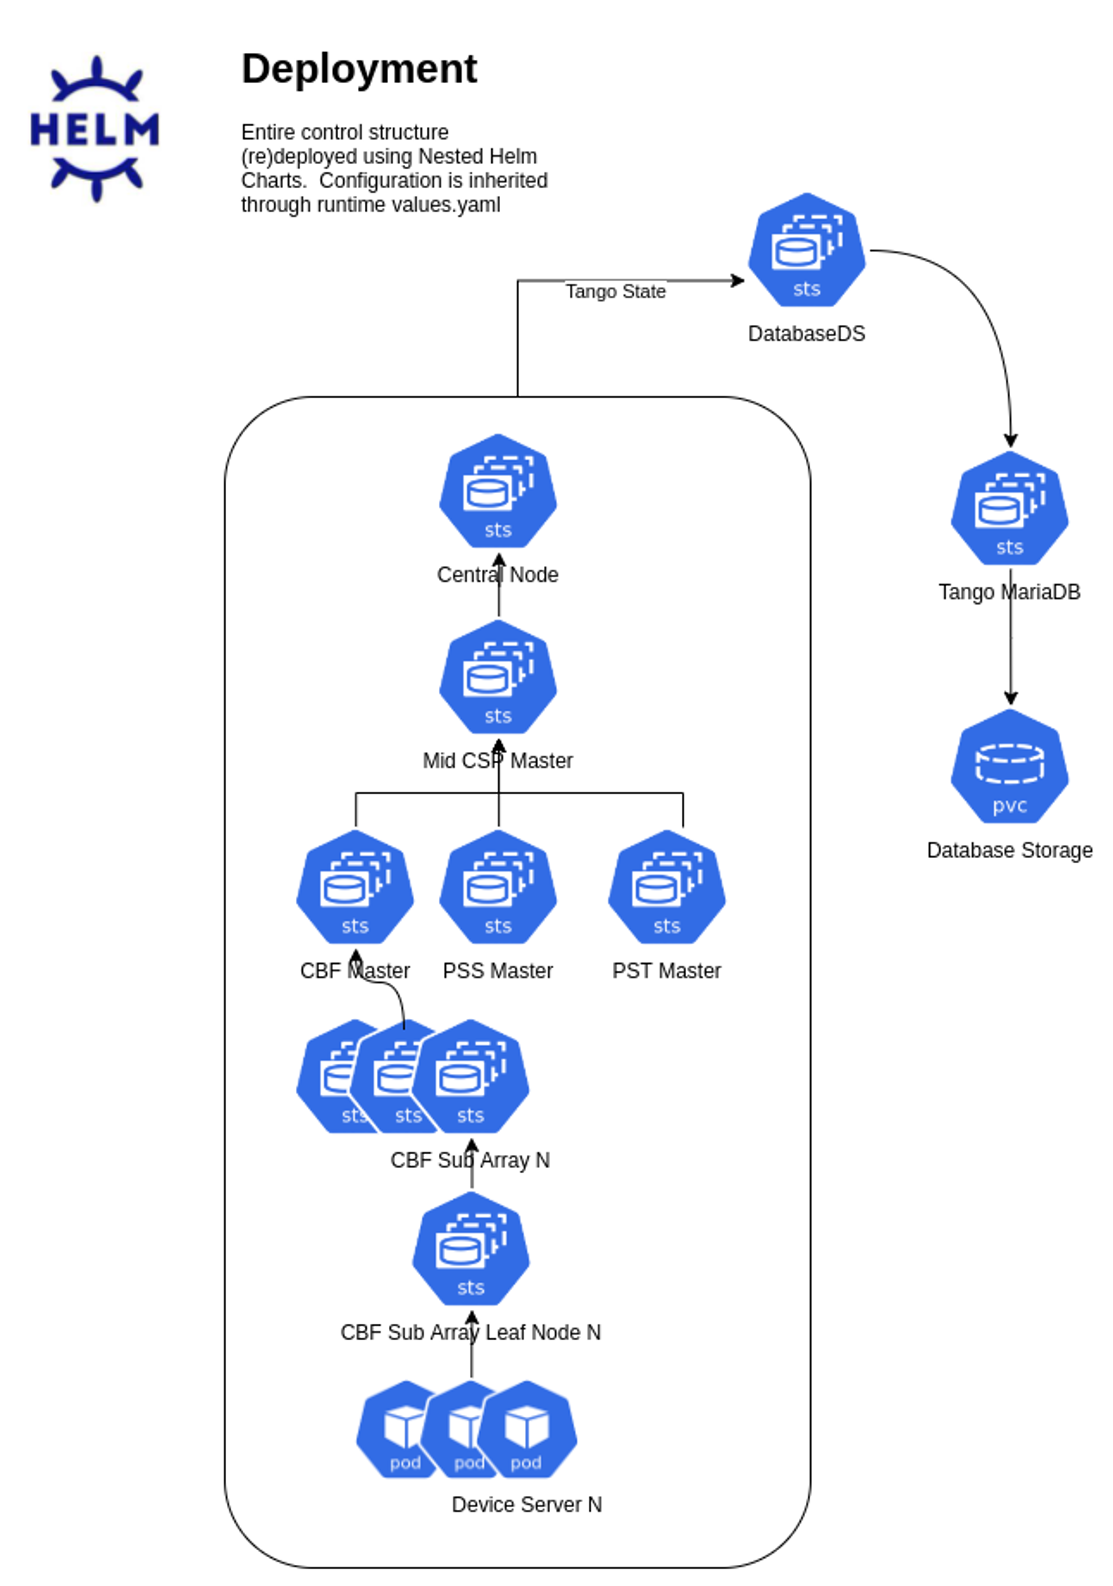
\includegraphics[height=16cm]{deployments.png}
   \end{tabular}
   \end{center}
   \caption 
%>>>> use \label inside caption to get Fig. number with \ref{}
   { \label{fig:deployment}
SKAO Kubernetes Deployment of a subsystem}
    \end{figure} 

\noindent\textbf{Initial CI/CD Deployment:} The first Minimum Viable Product (MVP) as shown in Figure \ref{fig:deployment} was deployed via continuous deployment (CD), showcasing the potential for automating deployment processes within the Kubernetes environment \cite{di_carlo_ci-cd_2020}. 

% Note: If compiling with LaTeX+dvipdf, please ensure images generated from 
% other software packages have their bounding boxes set correctly.
   \begin{figure} [ht]
   \begin{center}
   \begin{tabular}{c} %% tabular useful for creating an array of images 
   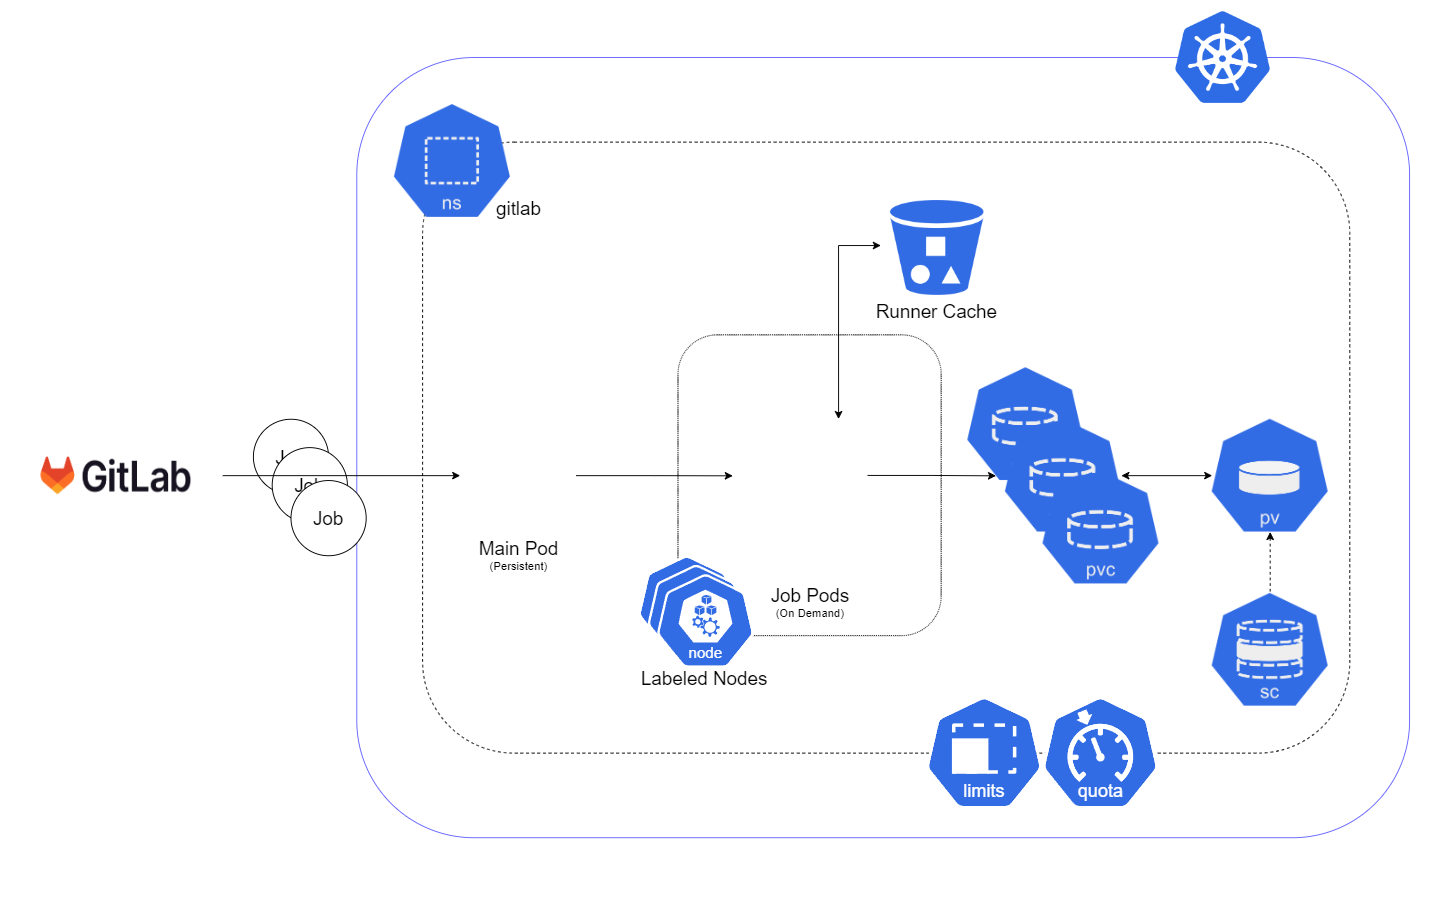
\includegraphics[height=10cm]{gitlab-runners.png}
   \end{tabular}
   \end{center}
   \caption 
%>>>> use \label inside caption to get Fig. number with \ref{}
   { \label{fig:runners}
SKAO Gitlab Runners on Kubernetes}
    \end{figure} 

\noindent\textbf{Migrating CI/CD Pipelines:} The next critical step was migrating existing CI/CD pipelines from VM/Shell runners into the Kubernetes cluster. This move facilitated better resource management and enhanced the scalability of the CI/CD processes. These runners were setup using Gitlab Kubernetes Executor with the architecture shown in Figure \ref{fig:runners}. 

\noindent\textbf{Logging and Monitoring:} Centralising logging and monitoring across multi cluster Kubernetes environments allowed for more efficient tracking and analysis of system performance and issues, significantly improving observability. It also allowed correlation and analysis of data across multiple environments to better highlight the issues and resource consumption.

\noindent\textbf{Automation of Software Development Lifecycle (SDLC)}: Automation extended to the entire SDLC for all projects, from code commit to deployment, enabling rapid iteration and deployment cycles. This also allowed developers to use out of the box solution with minimal overhead as a managed service where following the best practices and security updates were done for them by default. This is called \textit{Pipeline Machinery}\cite{team_skao_2024}

\noindent\textbf{Dynamic Environment Provisioning:} Automated provisioning and tear-down of environments based on CI/CD pipeline requirements allowed for efficient use of resources and facilitated faster testing and deployment cycles. This in conjunction with the above steps allowed streamlined and fast development turnout. The release management is also automated and tied to this machinery via usage of git tags. The release system then updated the correct files for versions and made sure the MR and documentation changes are followed on.

\noindent\textbf{ClusterAPI Integration:} The integration of ClusterAPI enabled the creation and management of multiple Kubernetes clusters with ease, further enhancing the scalability and flexibility of the CI/CD framework.

\noindent\textbf{Cloud Transition and Repatriation:} Temporary migration of all CI/CD processes to AWS demonstrated the portability and robustness of the cloud-native setup, followed by a seamless transition back to the original infrastructure when needed.

\subsubsection{Benefits of Cloud-Native CI/CD}

The journey to a cloud-native CI/CD framework has yielded several key benefits:

\begin{itemize}
    \item \textbf{Early Detection and Fast Feedback:} Continuous integration testing allows for the early detection of issues and provides rapid feedback to developers, reducing the time to resolve problems.
    \item \textbf{Clear Separation of Responsibilities:} Defined roles and responsibilities within the CI/CD pipeline ensure efficient management and clear accountability.
    \item \textbf{Scalability and Flexibility:} Kubernetes' hierarchical control structure and dynamic resource management capabilities enable the system to scale efficiently and handle complex workflows.
    \item \textbf{Enhanced Collaboration and Observability:} Improved monitoring and logging capabilities foster better collaboration among development teams and increase transparency in the deployment process.
\end{itemize}

\section{Platform Layered View}

% Note: If compiling with LaTeX+dvipdf, please ensure images generated from 
% other software packages have their bounding boxes set correctly.
   \begin{figure} [ht]
   \begin{center}
   \begin{tabular}{c} %% tabular useful for creating an array of images 
   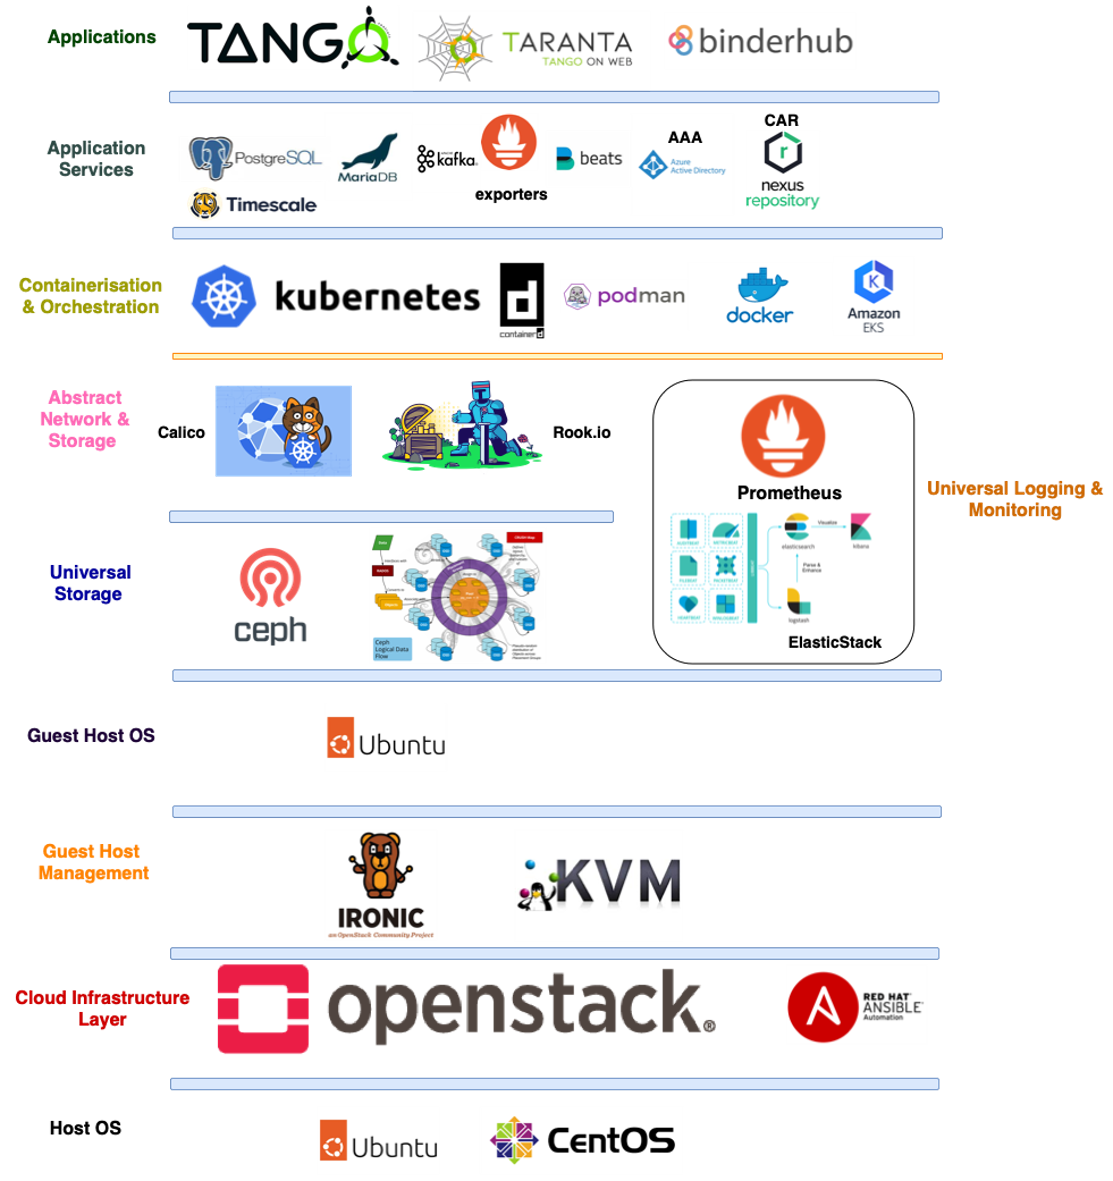
\includegraphics[height=16cm]{layers.png}
   \end{tabular}
   \end{center}
   \caption 
%>>>> use \label inside caption to get Fig. number with \ref{}
   { \label{fig:platform}
SKAO Platform Layered Approach (Not an exhaustive list) }
    \end{figure} 
    
The SKAO platform is structured into multiple layers, each designed to handle specific aspects of the CI/CD process, from infrastructure management to application deployment. This layered approach ensures a clear separation of concerns, allowing for better manageability, scalability, and flexibility. The primary layers include the infrastructure layer, orchestration layer, and application layer, each playing a crucial role in the overall system. Some important notes about the view are:

\begin{itemize}
    \item Different platform instances are possible, based on this stack. Not all platform instances will provide all the elements in this stack.
    \item Layers in this stack are optional, not all layers have to be present in all platform instances
    \item The layering is mainly used in this view as a grouping concept, making it easy for the reader to identify key elements. Different instances of the platform may present a different ordering in a layered representation.
\end{itemize}

\subsection{Infrastructure Layers}

At the base of the platform is the infrastructure layers, responsible for providing the foundational compute, storage, and network resources necessary for running applications. These layers are abstracted through Kubernetes, allowing developers to focus on higher-level functionalities without being bogged down by hardware complexities. Key components of the infrastructure layers include:

\begin{itemize}
    \item \textbf{Compute Resources:} Virtual machines and containerised environments that provide the necessary processing power for running applications and CI/CD pipelines.
    \item \textbf{Storage Solutions:} Persistent and ephemeral storage options to meet the varying data retention and performance requirements of different applications.
    \item \textbf{Networking Capabilities: }Advanced networking features that ensure seamless communication between containers, services, and external systems.
\end{itemize}

\subsection{Containerisation and Orchestration Layer}

The containerisation and orchestration layers are the heart of the SKAO platform, built on Kubernetes. They provide powerful tools for managing the deployment, scaling, and operations of containerised applications. These layers abstract the complexities of the underlying infrastructure, offering a cohesive and manageable interface for developers and operators. Key functionalities include:

\begin{itemize}
    \item \textbf{Resource Scheduling and Management:} Kubernetes ensures efficient scheduling of compute resources, balancing load, and optimising resource usage.
    \item \textbf{Service Discovery and Load Balancing:} Automatic detection and routing of services ensure high availability and reliability.
    \item \textbf{Configuration Management:} Helm charts and Kubernetes manifests are used to define and manage application configurations, allowing for consistent and repeatable deployments.
    \item \textbf{Custom Operators:} These are used to automate complex operational tasks and manage the lifecycle of specific applications, providing advanced capabilities tailored to the needs of SKAO.
\end{itemize}

\subsection{Application and Services Layers}

The application and services layers comprise the actual software applications and services that run on top of the orchestrated infrastructure. These layers benefits from the abstractions and services provided by the underlying layers, enabling seamless integration and efficient operations. Key aspects of the application layer include:

\begin{itemize}
    \item \textbf{Decoupled Deployments:} Applications are deployed as independent microservices or nested Helm charts, allowing for modular and flexible updates.
    \item \textbf{Runtime Configuration Injection:} Dynamic configuration management at runtime ensures that applications can adapt to changing conditions and requirements without downtime.
    \item \textbf{Operational Lifecycle Management:} Continuous monitoring, logging, and observability tools are integrated into the application lifecycle, providing insights and ensuring operational stability.
\end{itemize}

\subsection{Benefits of the Layered Approach}

The layered architecture of the SKAO platform offers several significant advantages:

\begin{itemize}
    \item \textbf{Scalability:} Each layer can scale independently, allowing for efficient resource management and handling of large-scale operations. Each layer is optional as not all platform instances will provide all the elements in the stack.
    \item \textbf{Flexibility:} Modular components and decoupled deployments enable rapid iteration and adaptation to changing requirements.
    \item \textbf{Transparency:} Clear separation of concerns and robust monitoring tools enhance visibility and accountability across the platform.
    \item \textbf{Manageability:} Abstractions provided by Kubernetes and custom operators simplify the management of complex workflows and operational tasks.
\end{itemize}

A practical example of the platform's layered approach is the integration of multi-cloud environments. By leveraging Kubernetes' abstraction capabilities, SKAO has successfully managed and orchestrated resources across different cloud providers, ensuring portability and flexibility. This integration allows SKAO to utilise the best features of various cloud platforms while maintaining a unified and cohesive operational framework.

\section{Continuous Integration and Continuous Deployment}

Continuous Integration (CI) and Continuous Deployment (CD) have been central to the SKAO’s software development lifecycle, enabling rapid development, testing, and deployment of software applications. The evolution of CI/CD practices at SKAO reflects a journey towards greater automation, efficiency, and scalability, underpinned by the adoption of cloud-native technologies. This process has been explained previously in more detail \cite{di_carlo_ci-cd_2020, yilmaz_driving_2023, team_skao_2024}. 

Initially, SKAO's CI/CD processes were manual and relied heavily on virtual machines (VMs) and shell runners. This setup posed several challenges:

\begin{itemize}
    \item \textbf{Manual Processes:} High manual effort was required for setup, configuration, and maintenance, leading to increased risk of human error and inefficiencies.
    \item \textbf{Limited Scalability:} VM-based pipelines struggled to scale with increasing workloads, resulting in slower build and deployment times.
    \item \textbf{Inconsistent Environments}: Variability in environments across different stages of the pipeline led to inconsistencies and integration issues.
\end{itemize}

Recognising the limitations of traditional methods, SKAO transitioned to a cloud-native CI/CD framework, leveraging Kubernetes to automate and streamline the entire process as shown in Figure \ref{fig:runners}. This transition involved several key steps and improvements:

\subsection{Cluster-Based CI/CD Pipelines}

Moving CI/CD pipelines into Kubernetes clusters allowed for better resource management and scaling. Kubernetes' inherent capabilities for container orchestration provided a robust foundation for automating build, test, and deployment stages.

By containerising CI/CD runners, SKAO ensured consistency and repeatability across different pipeline stages, reducing environment-related issues.

\subsection{Automated Environment Provisioning}

Implementing automated environment provisioning enabled on-demand creation and tear-down of testing and staging environments. This approach significantly reduced the time and effort required for environment setup, facilitating faster testing cycles.

Automated provisioning allowed the CI/CD system to scale dynamically based on workload demands, optimising resource usage and improving efficiency.

\subsection{Enhanced Monitoring and Logging}

Integrating centralised logging and monitoring solutions within Kubernetes containers provided comprehensive visibility into pipeline operations. This integration allowed for real-time tracking of system performance, facilitating quicker detection and resolution of issues. Enhanced observability through detailed metrics and logs helped in maintaining the reliability and stability of the CI/CD pipelines. 

The adoption of cloud-native CI/CD practices has enabled SKAO to implement several advanced capabilities:

\textbf{Integration Testing:} Automated integration testing ensures that independently developed subsystems work seamlessly together, reducing integration issues and improving software quality.

\textbf{Continuous Testing:} Continuous testing at various stages of the CI/CD pipeline provides rapid feedback to developers, enabling early detection and resolution of bugs.

\textbf{Operational Lifecycle Management: }Custom Kubernetes operators automate complex operational tasks and manage the lifecycle of specific applications, ensuring consistent and reliable operations. SKAO developed its own set of operators to work with Tango Controls Framework.\cite{controls_tango_home_2024}

\subsection{Stages and Environments of CI/CD Process}

Figure \ref{fig:envs} shows different tiers of environments SKAO manages through out SDLC.

% Note: If compiling with LaTeX+dvipdf, please ensure images generated from 
% other software packages have their bounding boxes set correctly.
   \begin{figure} [ht]
   \begin{center}
   \begin{tabular}{c} %% tabular useful for creating an array of images 
   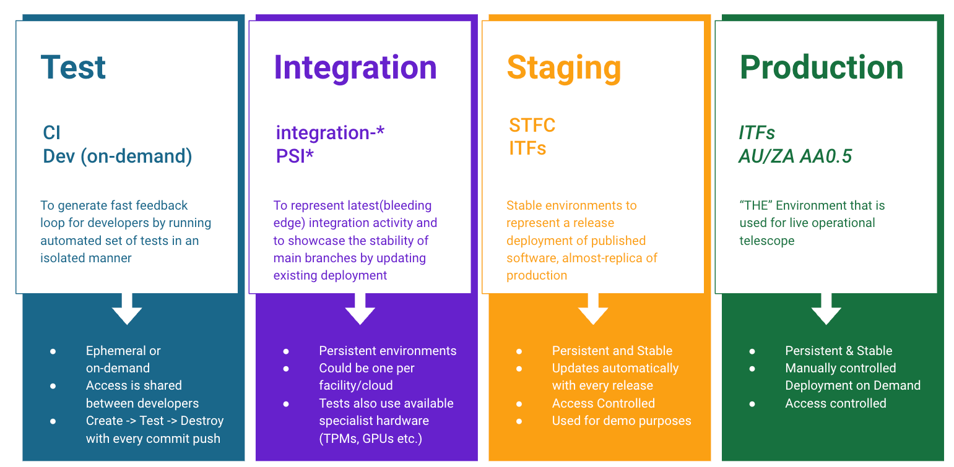
\includegraphics[height=8cm]{envs.png}
   \end{tabular}
   \end{center}
   \caption 
%>>>> use \label inside caption to get Fig. number with \ref{}
   { \label{fig:envs}
SKAO Software Environments }
    \end{figure} 

\subsubsection*{Test (CI/Dev (On-Demand))}

\begin{itemize}
    \item \textbf{Purpose}: This tier is designed to generate fast feedback for developers by running automated sets of tests in an isolated manner. It helps in identifying and fixing issues early in the development process.
    \item \textbf{Environment}: Ephemeral or on-demand environments are created and shared among developers. These environments are temporary and are destroyed with every commit push.
    \item \textbf{Activities}:
    \begin{itemize}
        \item Quick tests to validate the new code changes.
        \item Ensuring that the basic functionalities work as expected before integrating with the main branches.
    \end{itemize}
\end{itemize}

\subsubsection*{Integration}

\begin{itemize}
    \item \textbf{Purpose}: This tier represents the latest (bleeding edge) integration activity and showcases the stability of main branches by updating existing deployments.
    \item \textbf{Environment}: Persistent environments that could be one per facility/cloud. These environments may also utilise available specialist hardware (e.g., TPMs, GPUs).
    \item \textbf{Activities}:
    \begin{itemize}
        \item More extensive testing, including integration tests that combine multiple components to ensure they work together.
        \item Continuous integration ensures that the code changes from different developers are regularly merged and tested.
    \end{itemize}
\end{itemize}

\subsubsection*{Staging}

\begin{itemize}
    \item \textbf{Purpose}: Staging environments are stable environments used to represent a release deployment of published software, almost a replica of production. This tier is crucial for final validation before moving to production.
    \item \textbf{Environment}: Persistent and stable environments that update automatically with every release. Access to these environments is controlled and used for demonstration purposes.
    \item \textbf{Activities}:
    \begin{itemize}
        \item Thorough testing to ensure the application performs well under production-like conditions.
        \item Final acceptance testing, performance testing, and user acceptance testing to ensure readiness for production deployment.
    \end{itemize}
\end{itemize}

\subsubsection*{Production}

\begin{itemize}
    \item \textbf{Purpose}: This is the final tier of environment where the software is deployed for live operations. The production environment must be stable and reliable to support real-time observatory operations.
    \item \textbf{Environment}: Persistent and stable environments, manually controlled with deployment on demand. This is the "THE" environment used for live operational telescope activities.
    \item \textbf{Activities}:
    \begin{itemize}
        \item Deployment of the software for actual use.
        \item Ongoing monitoring and health checks to ensure system reliability and performance.
        \item Automated deployment and rollback mechanisms to manage updates and handle issues swiftly.
    \end{itemize}
\end{itemize}

\subsection*{CI/CD Pipeline Flow}

% Note: If compiling with LaTeX+dvipdf, please ensure images generated from 
% other software packages have their bounding boxes set correctly.
   \begin{figure} [ht]
   \begin{center}
   \begin{tabular}{c} %% tabular useful for creating an array of images 
   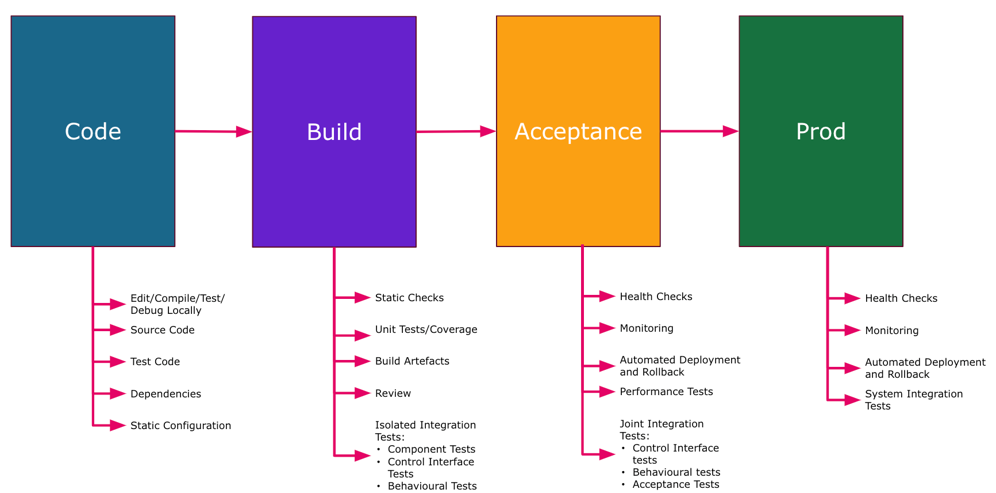
\includegraphics[height=8cm]{stages.png}
   \end{tabular}
   \end{center}
   \caption 
%>>>> use \label inside caption to get Fig. number with \ref{}
   { \label{fig:stages}
SKAO CI/CD Stages }
    \end{figure} 

The bottom part of the Figure \ref{fig:stages} depicts the CI/CD pipeline flow, showing the progression of activities from code development to production deployment:

\subsubsection*{Code}

\begin{itemize}
    \item Developers edit, compile, test, and debug code locally.
    \item Source code management, testing code, managing dependencies, and configuring static settings are done locally or on any development environment.
\end{itemize}

\subsubsection*{Build}

\begin{itemize}
    \item Performing static checks, unit tests, and coverage analysis as part of CI is done in this stage.
    \item Creating build artefacts and reviewing code is done before merging different works.
    \item Conducting isolated integration tests, including component and control interface tests are done to ensure functionality.
\end{itemize}

\subsubsection*{Acceptance}

\begin{itemize}
    \item Conducting health checks and monitoring to identify issues earlier.
    \item Automated deployment and rollback procedures are in place to ensure fast turnout and feedback.
    \item Performance testing and joint integration tests, including behavioural and acceptance tests are carried out.
\end{itemize}

\subsubsection*{Prod}

\begin{itemize}
    \item Conducting health checks and monitoring to identity and alert to any issues.
    \item Automated deployment and rollback procedures are in place to ensure the stability of production environment.
    \item Performing systems integration tests to ensure everything works together seamlessly in the live environment.
\end{itemize}

The Figures \ref{fig:envs},\ref{fig:stages} collectively illustrate the structured approach SKAO employs for its CI/CD process. By progressing through the stages of Test, Integration, Staging, and Production, SKAO ensures that software is developed, tested, and deployed efficiently and reliably. Each stage serves a specific purpose and is crucial for maintaining the stability and performance of the overall system, especially for large-scale and complex projects like SKAO.


\subsection{Key Metrics and Achievements}

The transition to a cloud-native CI/CD framework has resulted in significant improvements in operational metrics:

\begin{itemize}
    \item \textbf{Pipeline Runs:} Over 24,000 pipeline runs in the past six months indicate a high level of automation and continuous integration activity.
    \item \textbf{Dynamic Resource Usage:} Utilising over 1,000 virtual CPUs dynamically demonstrates the system's scalability and efficient resource management.
    \item \textbf{Deployment Efficiency:} Achieving more than 1,500 deployments highlights the effectiveness and reliability of the automated deployment processes.
\end{itemize}

\section{Conclusion}

 \subsection{Results}
 
The journey of the Square Kilometre Array Observatory (SKAO) in adopting cloud-native CI/CD practices has been marked by significant achievements and transformative outcomes. Key results from this journey include:

\begin{itemize}
    \item \textbf{Enhanced Automation:} The integration of Kubernetes into the CI/CD pipeline has automated numerous processes, from environment provisioning to deployment, significantly reducing manual effort and errors.
    \item \textbf{Scalability and Flexibility:} The ability to dynamically manage resources and scale operations based on real-time demands has improved efficiency and responsiveness to changing needs of the project.
    \item \textbf{Improved Reliability and Stability:} Centralised logging, monitoring, and enhanced observability have led to more stable and reliable operations, with quicker detection and resolution of issues.
    \item \textbf{Increased Deployment Velocity:} Over 24,000 pipeline runs and more than 1,500 deployments in the past six months highlight the high velocity and efficiency of the automated deployment processes.
    \item \textbf{Seamless Integration:} The use of advanced CI/CD capabilities, such as automated testing and custom operators, has ensured seamless integration of independently developed subsystems, enhancing overall software quality.
\end{itemize}

\subsection{Lessons Learned}

Throughout this journey, several important lessons have been learned that are also mentioned in SAFe Framework\cite{safe}:

\begin{itemize}
    \item \textbf{Continuous Improvement:} Adopting cloud-native technologies is an ongoing process that requires continuous adaptation and refinement to meet evolving needs and challenges.
    \item \textbf{Collaboration and Transparency:} Improved collaboration and transparency, facilitated by enhanced monitoring and logging, are crucial for the success of large-scale projects.
    \item \textbf{Resource Management:} Efficient resource management and dynamic provisioning are key to maintaining scalability and flexibility in a complex CI/CD environment.
\end{itemize}

\subsection{Future Work}

Building on the success of the current cloud-native CI/CD framework, SKAO plans to focus on several areas for future enhancement:

\textbf{Gradual Stabilisation:} Continue to stabilise and optimise the CI/CD processes, ensuring robust compatibility and reliability across different environments. Implement performance tuning measures to further enhance the efficiency and speed of the CI/CD pipelines.

\textbf{Enhanced Deployment Mechanisms:} Explore and implement more advanced deployment strategies, such as blue-green deployments, pull based deployments and A/B testing, to further minimise downtime and deployment risks.

\textbf{Multi-Cloud Strategy:} Continue to expand and refine the multi-cloud strategy, leveraging the best features of various cloud providers while maintaining a unified operational framework.

\textbf{Cloud-Native Security:} Enhance security measures within the multi-cloud environment, ensuring data integrity and protection across all platforms.

\textbf{Community Collaboration:} Foster collaboration with other organisations and research institutions to exchange knowledge and best practices, driving further innovation in cloud-native CI/CD practices.

The adoption of cloud-native CI/CD practices at SKAO has been a transformative journey, yielding significant improvements in automation, scalability, reliability, and deployment velocity. By leveraging Kubernetes and other cloud-native technologies, SKAO has built a robust and efficient CI/CD framework that supports its ambitious scientific goals. As SKAO continues to evolve and enhance its CI/CD practices, it remains committed to pushing the boundaries of astronomical research and technological innovation, paving the way for future advancements in large-scale scientific projects.

% References
\bibliography{report} % bibliography data in report.bib
\bibliographystyle{spiebib} % makes bibtex use spiebib.bst

\end{document} 